\section{Introduction}
\label{sec:introduction}

Provenance graph as a threat representation tool are already widely studied and adopted \cite{li2021}. With provenance graph, security analyzers are able to encode system execution history into graphs. Thus provenance graph contain rich semantic information. However, there are still a gap between provenance graphs and human understandable information. Poirot \cite{Milajerdi2019} try to solve this problem by involve TTPs and kill chain proposed by MITRE \cite{}.

\begin{figure}
    \centering
    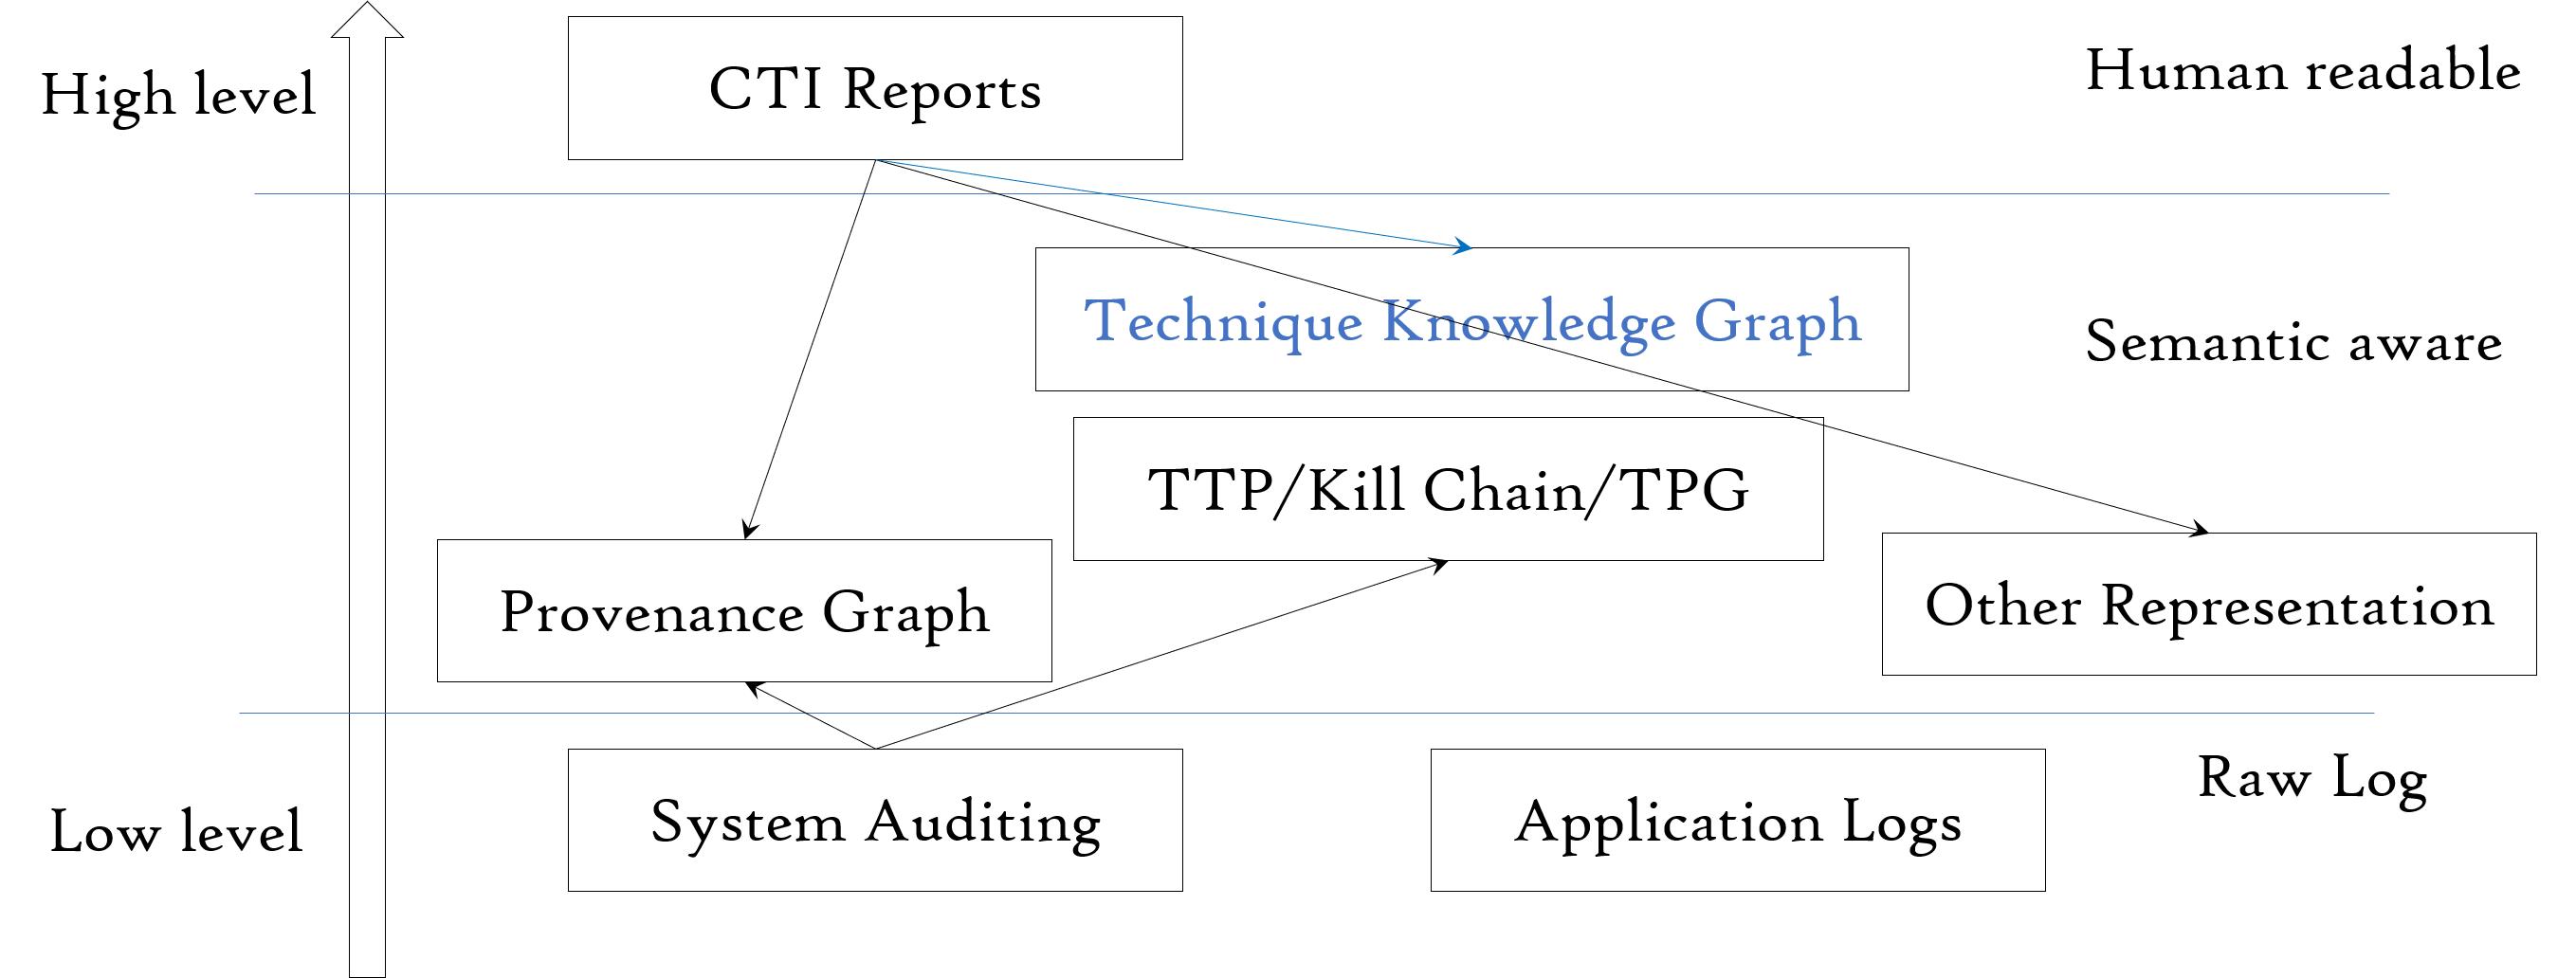
\includegraphics[width=3.5in]{Image/representation.png}
    \caption{Different Representation of Cyber Attacks.}
    \label{fig:representation}
\end{figure}

